\chapter{Methods}
In this chapter of the thesis are described methods that can be applied to the detection of the bricks. Only a brief description is provided, and all methods are presented in a general form.

\section{Lidar detection range analysis}
It is useful to know a possible range of detection based on the lidar sensor. This range influences how the robot explores the arena and influences the choice of used methods. Higher the detection range is, a lower number of waypoints is necessary to explore the whole arena. There is a limited time for exploration because brick pickup and brick placement take much time. The speed of pickup and placement is limited mainly by the speed of the Kinova arm. We estimate the maximal range using the Figure \ref{fig:range}.

\begin{figure}[H]
	\centering
	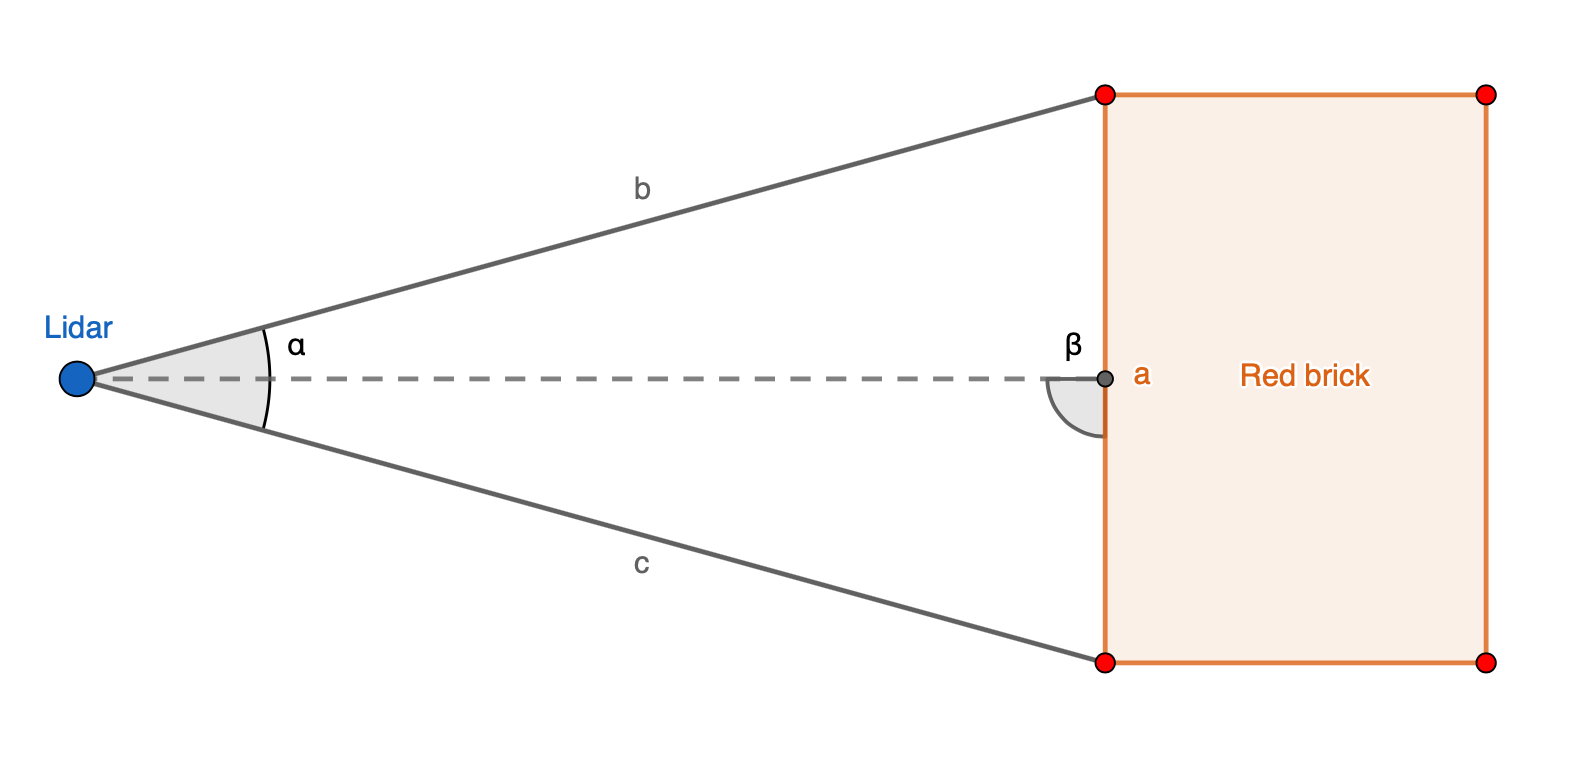
\includegraphics[scale=1.1]{fig/lidar_range.png}
	\caption[Lidar range study]{Visualization of rays hitting the red brick.}
	\label{fig:range}
\end{figure}

Angle $\alpha$ is the resolution of lidar known from table \ref{tab:lidar}. Only the maximal range is calculated, thus angle $\beta = 90\degree$. The cosine theorem can be used to obtain the distance between points on the brick.
\begin{equation}
a^2 = b^2 + c^2 - 2bc \cos \alpha.
\end{equation}
Because $\beta$ is right angle we can write $b = c$ and thus:
\begin{equation}
a = \sqrt{2b^2 \left(1-\cos \alpha \right)}.
\end{equation}
Now we want to know how many rays $N$ would hit the brick from given distance $b$ with lidar angular resolution $\alpha$ and the size of the brick $a$. 
\begin{align}
a &= \sqrt{2b^2 \left(1-\cos \left( N \alpha \right) \right)}, \\
N &= \frac{\arccos\left(1-\frac{a^2}{2b^2}\right) }{\alpha}.
\label{eq:rays}
\end{align}
Finally, we can plot a function of the number of rays $N$ with respect to distance to object $b$. This analysis can be done similarly for vertical and horizontal resolution.

\begin{figure}[H]
	\centering
	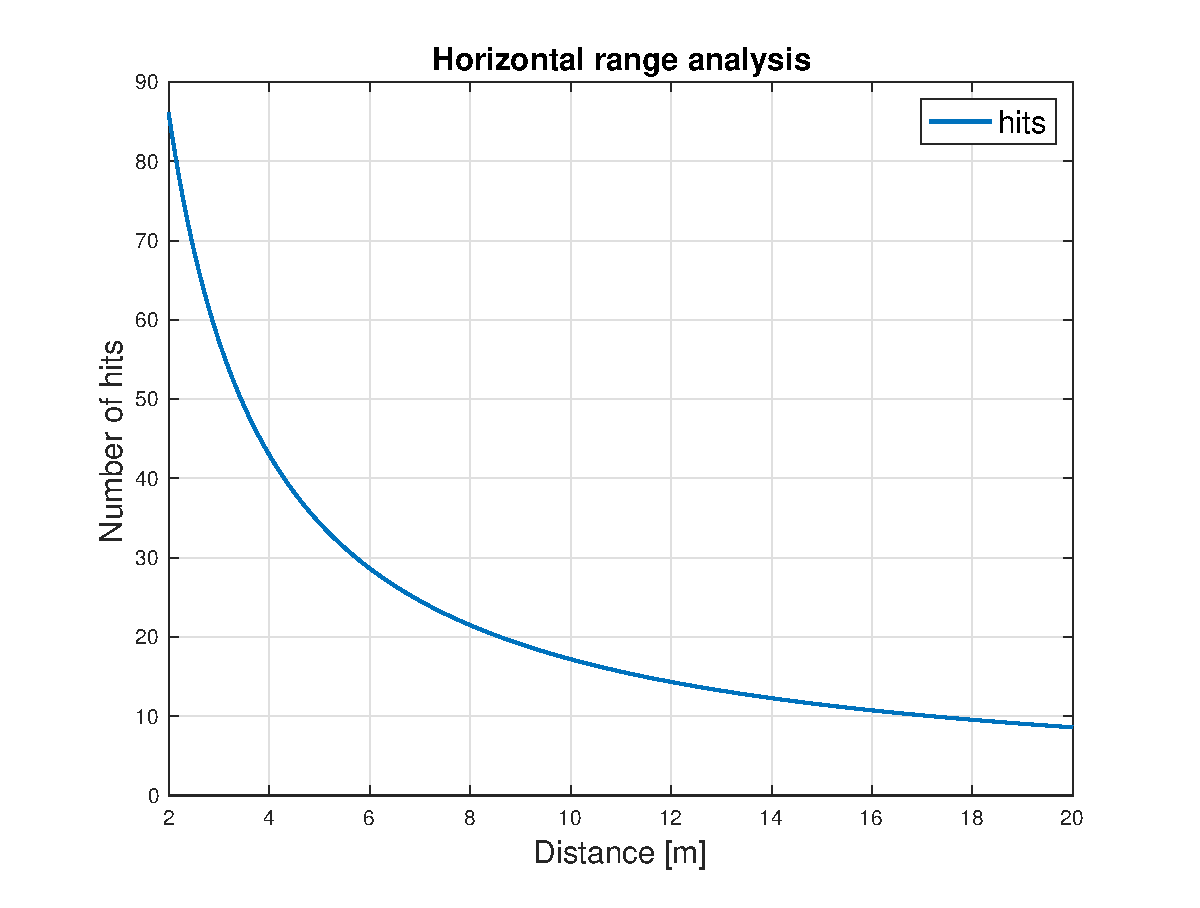
\includegraphics[scale=0.55]{fig/horizontal_range.eps}
	\caption[Horizontal range chart]{Number of rays which hits the smallest brick from given distance.}
	\label{fig:horizontal_hits}
\end{figure}

In Figure \ref{fig:horizontal_hits} is visible that the horizontal resolution of the lidar is not limiting factor of the range. Even from 10 meters is lidar able to hit red brick more than 15 times. On the other hand, the Figure \ref{fig:vertical_hits} shows that less than two lidar layers would hit the pile of bricks with a height of 40 cm from a distance greater than 6 meters. Furthermore, this is the best-case scenario analysis where $\beta$ is a right angle, which rarely happens in reality.

\begin{figure}[H]
	\centering
	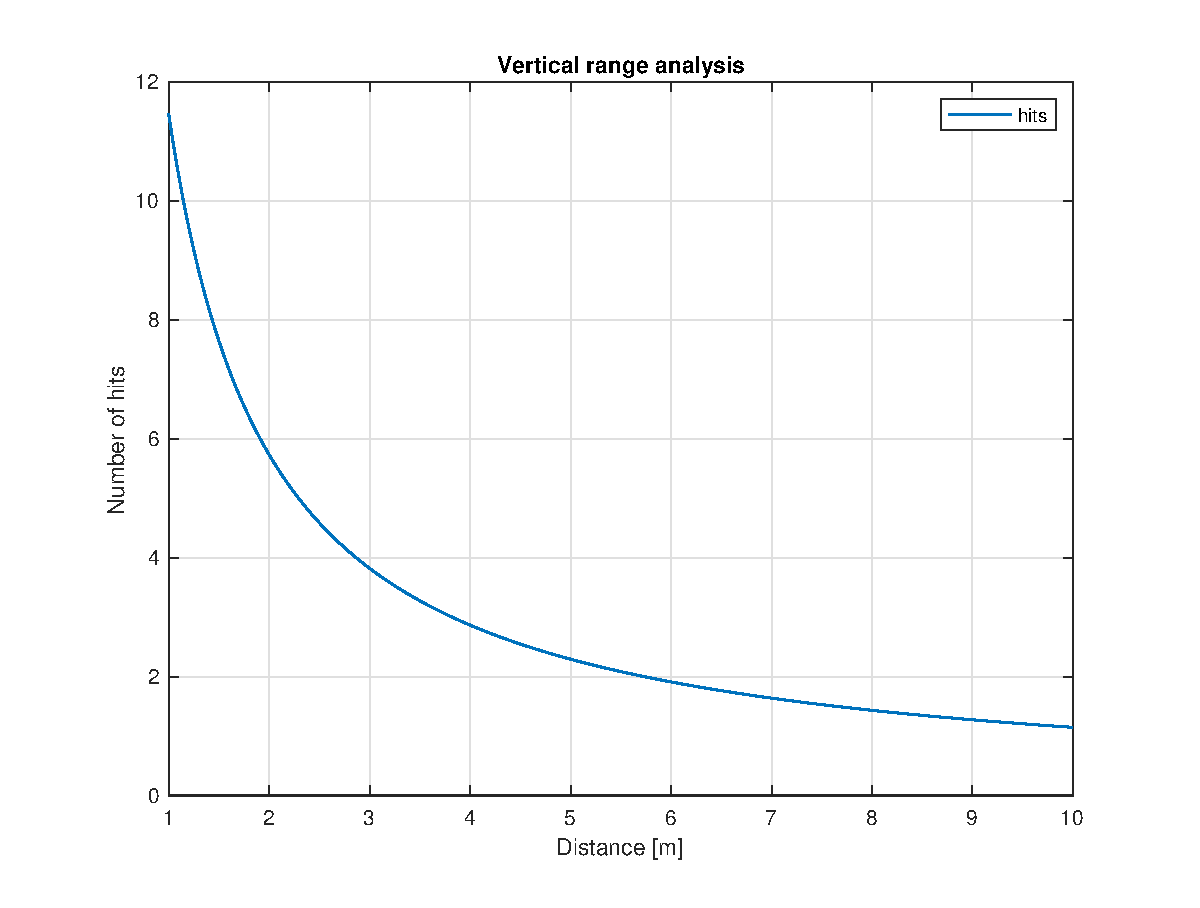
\includegraphics[scale=0.55]{fig/vertical_range.eps}
	\caption[Vertical range chart]{Number of layers which hits two stacked bricks from given distance.}
	\label{fig:vertical_hits}
\end{figure}

\section{Lidar data processing}

It would be handy to extract straight lines from lidar data to detect individual bricks. Several methods can be used to achieve this goal. One of the most popular algorithms for line extraction is currently split and merge algorithm. Initially was this algorithm proposed for image segmentation by Horowitz and Pavlidis \cite{horowitz1976}. A simple version of this algorithm for point-cloud processing is described in algorithm \ref{alg:segmentation}, where C is clustering distance and S is splitting distance. There are many implementations of this algorithm which differ mainly in a way how they compute some particular steps of the algorithm. For example, just the method of fitting a line to the cluster can vary a lot. The method of least squares is often used, but as a simple method as connecting endpoints of the cluster could be used. When the latter method is applied, the algorithm is usually referred to as Iterative End Point Fit (IEPF) \cite{siadat1997}. For the cluster creation, the points are iterated in each layer one by one. When the distance of the following points is too high, we split the cluster. Every cluster is then further recursively split based on the most distant point from the fitted line. In comparison to other line extraction algorithms is the split and merge algorithm, one of the best performings in terms of precision and computational complexity \cite{nguyen2006}.
\begin{algorithm}[]
 \KwData{pointcloud}
 \KwResult{line\_segments}
initialize constants C, S\;
  clusters = find\_clusters(pointcloud, C)\;
\While{clusters is not empty}{
	cluster = clusters.pop()\;
	line = fit\_line(cluster)\;
	point = most\_distant\_point(cluster, line)\;
	\eIf{distance(point, line) $>$ S}{
	   c1, c2 = split\_cluster(cluster, point)\;
		clusters.push\_back(c1, c2)\;
	}{
		line\_segments.push\_back(cluster[start], cluster[end])\;	
	}
}
merge\_parallel(line\_segments)\;
 
 \caption{Lidar data segmentation using split and merge algorithm.}
 \label{alg:segmentation}
\end{algorithm}


\section{EM algorithm}
Expectation-maximization (EM) algorithm is an iterative process that can find parameters of a specified statistical model based on incomplete data. One of the most used statistical description for the EM algorithm is the Gaussian mixture model. This model is particularly useful because it emerges in many real-world situations, and it is easy to maximize. As the name of the algorithm suggests, it repeats the expectation and maximization step. Each iteration of the algorithm should improve the likelihood of the model until the terminating criterion is met. The termination criterion can simply be the number of iterations, or the algorithm can be stopped when the model is not improving anymore. Although we are discussing mainly the Gaussian distribution, the EM algorithm can also be used for other distributions from exponential family \cite{dempster1977}. The usage of the EM algorithm for the classification of 3D lidar data is not an entirely novel approach. Gaussian mixtures were already used for terrain recognition \cite{lalonde2006}.
 
\subsection{Maximization}
For maximization step is used maximal likelihood estimate weighted by $\gamma$ from expectation step. For parameters of Gaussian distribution $\mathcal{N}(\mu, \sigma)$ and number of samples $N$ looks maximization as follows:
\begin{equation}
\mu = \sum_{n = 1}^{N} \gamma_n x_n, \\
\end{equation}
\begin{equation}
\sigma = \sum_{n = 1}^{N}\gamma_n (x_n - \mu)^2 .
\end{equation}

A critical assumption for the convergence of the algorithm is that its likelihood with respect to the estimated parameter must be concave. This can be easily proved by computing the second derivative of the likelihood function. For example, for the mean value of distribution  $\mu$, it is easy to show that the second derivative of likelihood is always negative, which means that the function has no local optima.
\begin{align}
\mathcal{L} &= \prod_{n=1}^N \mathcal{N}(x_n, \mu, \sigma), \nonumber \\
\frac{\partial \log \mathcal{L}}{\partial \mu} &= \frac{1}{\sigma^2} \sum_{n = 1}^{N} (x_n - \mu), \\
\frac{\partial^2 \log \mathcal{L}}{\partial \mu^2} &= \frac{-N}{\sigma^2}. \nonumber
\end{align}

\subsection{Expectation}
The expectation step is done simply by evaluating conditional probability of current parameters given the sample:
\begin{equation}
\gamma_n = P(\mu, \sigma | x_n),
\end{equation}
which is calculated using the Bayes theorem and the law of total probability:
\begin{align}
\gamma_n &= \dfrac{P(x_n | \mu, \sigma) P(\mu, \sigma)}{P(x_n)}, \nonumber \\
\gamma_n &= \dfrac{P(x_n | \mu, \sigma) P(\mu, \sigma)}{\sum_{k = 1}^N P(x_k | \mu, \sigma) P(\mu, \sigma)}.
\end{align}
There is only one class so the priors can be evaluated $P(\mu, \sigma) = 1$ and the equation simplifies to final form:
\begin{equation}
\gamma_n = \dfrac{\mathcal{N}(x_n, \mu, \sigma) }{\sum_{k = 1}^N \mathcal{N}(x_k, \mu, \sigma) }.
\end{equation}

\subsection{Algorithm}
How to implement a generic version of the EM algorithm on sampled data is shown in algorithm \ref{alg:em}, where \textbf{x} is the observed data samples. All relevant calculations for Gaussian distribution are described in previous subsections. It is not clear where to start iterating. It is possible to start both with the expectation and with the maximization step, but both parts are dependent on the result of the other one. Here we start with the maximization step, so during the initialization, we set $\alpha_n = 1$. If some prior information about the model's parameters is available, they can be set during the initialization, and the algorithm can be started with the expectation step. This informed initialization can remarkably reduce the number of iterations and sometimes even an outcome of the algorithm.
\begin{algorithm}[]
 \KwData{x}
 \KwResult{parameters $\theta$}
 set all $\alpha_n$ = 1\;
\While{not stopping\_criterion(x, $\theta$)}{
	$\theta$ = maximization(x, $\alpha$)\;
	$\alpha$ = expectation(x, $\theta$)\;
} 
 \caption{Pseudocode shows how to implement the EM algorithm.}
 \label{alg:em}
\end{algorithm}


\section{RANSAC}
Random sample consensus (RANSAC) is an iterative method which can estimate parameters of the hypothesis given the data. It was first presented by Fischler \cite{fischler1981} with application in scene and image analysis, but it can be used for fitting arbitrary hypothesis. The most significant advantage of this algorithm is its robustness to outliers. The major drawback of this method is its high time complexity when fitting hypotheses to noisy data with a large number of samples. The whole iterative process is described in the algorithm \ref{alg:ransac}, where x is the observed data, $\eta$ is the maximized cost and $\theta$ are the parameters of the hypothesis.
\begin{algorithm}[]
 \KwData{x}
 \KwResult{best parameters $\theta^*$}
 initialize $\theta, \theta^*, \eta, \eta^*$\;
\While{not stopping\_criterion(x, $\theta$)}{
	samples = draw\_samples(x)\;
	$\theta$ = find\_parameters(samples)\;
	$\eta$ = compute\_cost(x, $\theta$)\;
	\If{$\eta > \eta^*$}{
		$\eta^* = \eta$\;
		$\theta^* = \theta$\;
	}
} 
 \caption{Pseudocode shows how to implement the RANSAC algorithm.}
 \label{alg:ransac}
\end{algorithm}

The number of drawn samples in \textbf{draw\_samples} must be equal or higher than the number of degrees of freedom of the hypothesis. After drawing the samples method, \textbf{find\_parameters} assigns the correspondences between sampled data and the hypothesis. The correspondences are used to obtain the parameters of the hypothesis. Then the algorithm is evaluating the quality of the hypothesis by applying the hypothesis to the whole dataset. This quality estimate can be done by an arbitrary cost function. A common practice is to define some metrics in our domain and use a threshold value to obtain the number of samples that fit the hypothesis. These samples are often referred to as inliers. Stopping criterion is usually met when the probability of sampling a better hypothesis is lower than a specified threshold. This section describes just the basic version of the algorithm. Many improvements to the RANSAC algorithm was proposed since 1981 \cite{chum2008}.

\subsection{Tentative Correspondences}
The tentative correspondences can help us to choose better samples from the data to generate a better hypothesis. It is necessary to define some function witch measure the similarity between data and hypothesis. The data which has a higher similarity to the hypothesis is then chosen with higher probability. It is also possible to completely ban correspondences with low similarity. Given the typical application in scene analysis, the similarity is usually computed by comparing keypoint descriptors.

\section{Global model and transformations}
One of the goals of this thesis is to develop a global model that can efficiently store and update the positions of interest points. This global model is in the map coordinate frame. The localization of the robot is essential for the precise global model. Every detection must be transformed from the coordinate frame of the sensor to the coordinate frame of the map. Transformation can be easily done using matrix multiplication:
\begin{equation}
\begin{bmatrix}
x^\prime \\
y^\prime \\
z^\prime 
\end{bmatrix}
=
R \begin{bmatrix}
x \\
y \\
z
\end{bmatrix}
+ \vec{t},
\end{equation}
where $R$ is $3\times3$ the rotation matrix and $\vec{t}$ is a $1\times3$ translation vector between coordinate frames. Similarly the transformation can be done in homogenous coordinates by merging translation and rotation into one matrix $T$:
\begin{equation}
\begin{bmatrix}
\vec{x^\prime} \\
1
\end{bmatrix}
=
\begin{bmatrix}
 \bm{R} & \vec{t} \\
 \vec{0} &  1
\end{bmatrix}
\begin{bmatrix}
\vec{x}\\
1
\end{bmatrix}.
\end{equation}

Different framework for computing the transformations is using quaternions. The quaternions are currently the standard for transformations in computer graphics and robotics. The most significant advantage of quaternions is that they are more efficient and do not suffer from gymbal lock and ambiguity of rotation. Arbitrary rotation and scaling can be expressed as quadruple of numbers in the quaternion framework. The rotation between coordinate frames $B \to A$ is computed with quaternions as:
\begin{equation}
q_A = q_T q_B q_T^*,
\end{equation}
where $q_A$ is quaternion in coordinate frame $A$, $q_B$ is quaternion in coordinate frame $B$, $q_T$ is quaternion representing the transformation between these coordinate frames, and $q_T^*$ is its conjugate. There is available a library within the ROS which can handle all these transformations in different forms \cite{tf}. 

\subsection{Symbolic map}
When all detections are transformed into the map frame, we can add them to a symbolic map. The symbolic map is storing the positions of all interest points and makes up the global model of the arena. Every object added to the symbolic map has a float number, which indicates the confidence of detection. When there is a new detection within a specific range from an object already stored in the symbolic map, a new object is not added, but only the confidence is increased. The range in which we just update the confidence is denoted as $cluster\_size$. This approach creates clusters of interest points of different types. All interest points can be polled from the symbolic map, and the robot can make decisions based on the confidence of such an interest point. The symbolic map also checks whether the inserted object is located inside the arena. Otherwise, the object is rejected. One of the features of such a map is that it does not have to rely on measurements just from one sensor and can contain entries based on different types of measurements \cite{majer2019}.

\subsection{Lidar to camera registration}
As can be seen in Figure \ref{fig:brickdef} (where the bricks are defined) besides the dimensions, another important feature of the bricks is their color. Although the color manifests itself a little bit in reflectivity of the surface, which can be detected by lidar, it is not possible to reliably distinguish the colors using only the lidar sensor. Until there is a gap between the individual bricks, it is possible to detect brick using just the spatial data. Ideally, the robot should be stacking bricks next to each other without any significant gap. Without any information about the color, it is impossible to decide whether the robot is detecting one large brick or several small bricks put together. So for this part of detection is necessary to color the point-cloud. Coloring can be done by using the image from Intel RealSense camera and projecting a 3D lidar point-cloud to the camera plane. For this purpose is used the pinhole camera model. To describe such a model is used intrinsic camera matrix $K$ which consists of intrinsic camera parameters \cite{hartley2017}
\begin{equation}
K = \begin{bmatrix}
f_x & 0 & c_x \\
0 & f_y & c_y \\
0 & 0 & 1
\end{bmatrix},
\end{equation}
where $f_x, f_y$ are focal lengths and $c_x, c_y$ stands for optical center of the camera.

Firstly is necessary to transform the whole point-cloud from the lidar coordinate frame to the camera frame. For this purpose, so-called extrinsic camera parameters are used, which describe where a camera is placed in the lidar coordinate frame. This type of transformation is discussed at the beginning of this section. Secondly, we can use the intrinsic camera parameters to calculate the projection. Note that it is needed to work in a homogenous 2D coordinate system.
\begin{equation}
\begin{bmatrix}
u\\
v\\
1
\end{bmatrix}
= K \begin{bmatrix}
x\\
y\\
z
\end{bmatrix}.
\end{equation}
It is possible to decide which coordinates $u,v$ on image plane corresponds to 3D point $x,y,z$ from point-cloud, and assign the color of a specific pixel to the point, using this matrix equality. However, this works only for the simplest pinhole camera model without any distortion of the image. If the lens has non-negligible distortion, this distortion must be included in the camera model. For the description of distortion are used the distortion coefficients.